\chapter{Implementation}
\label{chapter:implementation}

% \emph{[- Embedded -  Trained Model deployment to embedded microcontroller, quantization, STM32 platform specifics, audio handling, NN model options]}
% \bigskip

After selecting the best performing models in this chapter we are aiming to run the inference with real-time data collection on an embedded microcontroller platform and finally assemble a real-time multisensory room occupancy detector, by interfacing with a PIR sensor and merge the predictions.

\section{Embedded hardware platform}

Choosing a specific company or product line for embedded software development has to be planned with great care. Chip manufacturers and prototype makers create their unique solutions and development environments making it exceptionally hard to switch platforms within the industry with the additional steep learning curve for application development. Our task involves audio processing, feature extraction, and machine learning inference just to mention the most computationally demanding ones. Moreover, trained models usually require a relatively large amount of memory for storing the weights and biases, therefore various techniques are developed to reduce the memory footprint by transferring the model parameters to lower resolution fixed-point numbers like in quantization or compress the model (weight sharing algorithm, K-means clustering, only for fully connected layers..).


Hardware requirements:
\begin{itemize}
    \item Deep Learning requirements: increased memory for model parameters (64KB+), FPU, DSP instructions 
    \item Digital audio processing requirements:  peripheral to memory DMA, I\textsuperscript{2}S bus, 16k sample rate option
\end{itemize}

\section{STMicroelectronics}

Based on the criteria described above the firm STMicroelectronics was chosen due to its wide portfolio of microprocessors and development boards in our target range and software support tools for fast prototyping such as project generation by CubeMX or machine learning model conversion by X-CUBE-AI. Among their development boards, we aimed to find a cost-efficient option with DSP and FPU with the necessary communication interfaces for a digital MEMS microphone. 


Software tools used for initial project generation:
\begin{itemize}
  \item  \textbf{STM32CubeMX} is an official graphical tool for microcontroller and interface peripheral configuration with C code generation for the selected environment. As a final result, the user can focus more on the application development given that the peripheral initialization and library compatibility issues are already resolved automatically. The tool enables the user to select the desired microcontroller or development board and configure the GPIO and clock settings in an assisted manner, while the pinout-conflict solver aims to spot when a pin is used for multiple purposes and suggest alternative options. Moreover, the software functionality can be extended with various expansion packages too, in our project the only the X-CUBE-AI add-on is used.
  \item  \textbf{X-CUBE-AI} is a STM32CubeMX Expansion Package for automatic conversion of pre-trained Deep Neural Networks and optimized library generation for AI projects. The tool expects a saved Tensorflow Lite, Keras, or ONNX model to convert it to an efficient C library for inference purposes only. It supports 8-bit model quantization for processors without FPU and model compression for fully connected layers only.
 \item  \textbf{STM32CubeIDE}: The STM32CubeIDE is ST's own Eclipse-based multi-OS supported Integrated Development Environment (IDE) for embedded microcontrollers. Rich programming and debugging features make it a truly versatile tool.
\end{itemize}  

  
Software libraries:
\begin{itemize}
  \item \textbf{CMSIS}: Cortex Microcontroller Software Interface Standard, developed by ARM, provides a generic API for all Arm Cortex processors, simplifying software reuse and maximizing the computational performance of chips. Functions from their DSP module are utilized for audio signal processing in this project while the CMSIS-NN module is used by the X-CUBE-AI tool for generating efficient neural network instances for inference. Arm-based research \cite{lai2018cmsisnn} shows that CMSIS-NN based kernels can demonstrate a significant amount of increase (2.5x to 5x) in throughput and energy efficiency compared to traditional approaches.
  % https://arxiv.org/pdf/1801.06601.pdf
  
  \item  \textbf{STM32 AI Audio Preprocessing library} is a generic C library for audio frequency domain analysis and feature extraction, such as spectrogram, mel-scaled spectrogram computation, and Mel-frequency cepstral coefficient (MFCC) extraction. Uses the CMSIS DSP library for runtime optimization.
  
  \item  \textbf{HAL library} is an acronym for Hardware Abstraction Layer. STM32 provides a generic, high-level, feature-oriented Application Programming Interface (API) for development, allowing portability across the company's various microcontroller options. The HAL library hides the complexity of the selected MCU and peripherals, therefore helps the engineer to focus on application-specific challenges.
  \item  \textbf{BSP drivers} or Board Support Package is a set of functions ready-made for the selected board based on the HAL drivers. The goal is to speed up the prototyping phase by providing the necessary configuration and interfacing endpoints for components and peripherals fixed on the development board. Examples contain LEDs user buttons, or other board-specific peripherals such as LCD, Audio, or Touchscreen. Configurations may be overwritten by the user if certain settings are not wanted, but it is only recommended after careful consideration since the hardware connections might cause undesired behavior.

\end{itemize}

%STM32 code sources
% https://www.st.com/content/st_com/en/ecosystems/stm32-ann.html
% https://www.st.com/en/embedded-software/fp-ai-sensing1.html
% https://github.com/anderslanders/stm32-smart-headphones

\subsection{STM32 Nucleo-64 board}

The selected prototyping board for testing is the Nucleo-F401RE. It is one of the top-end models of the Nucleo-64 high-performance product line with an integrated ST-LINK debugger, programmer, and virtual COM port, allowing the user to start the development easily by connecting it to the computer with a single USB cable. 



\begin{table}[h!]
\begin{tabular}{|l|l|}
\hline
\textbf{Feature}                  & \textbf{STM32F401RE}             \\ \hline
Clock frequency                   & 84 MHz                           \\ \hline
Flash                             & 512 KB                           \\ \hline
SRAM                              & 96 KB                            \\ \hline
FPU                               & Available                        \\ \hline
Cache                             & None                             \\ \hline
Adaptive Real-time Accelerator(ART)    & Available                   \\ \hline
Timers                            & 11 Timers                        \\ \hline
DMA controllers                   & 2 DMAs                        \\ \hline
UART                              & 3 USARTs                         \\ \hline
Serial Peripheral Interface (SPI) & 4 SPIs (2 I\textsuperscript{2}Ss can be configured) \\ \hline
USB Interface                     & 1 USB 2.0                        \\ \hline
\end{tabular}

\caption{STM32 microcontroller specification summary.}
\end{table}


\subsection{Peripherals}

In the next sections, the selected hardware peripherals and their interfacing options with the selected microcontroller will be elaborated. Most importantly the audio and the PIR sensor properties and applicability for the test use case and the necessary Digital Signal Processing steps as a prerequisite for matching the input for the machine learning inference.


\subsubsection{Audio sensor}
\label{subsub:Aud_sensor}

The chosen audio sensor for the embedded implementation is the Adafruit I\textsuperscript{2}S MEMS Microphone Breakout board with a Knowles SPH0645LM4H MEMS Digital Microphone. The advantage of using an I\textsuperscript{2}S digital microphone over an analog version, is the compactness of the solution, quick prototyping results, and the direct connection with the MCU without an external audio codec. On the other hand, an inherent disadvantage of such compact boards that it does not give any room for customization, additional analog filtering or just to access the raw analog microphone signal is impossible.


\begin{table}[h!]
\centering
\begin{adjustbox}{max width=1\textwidth}
\begin{tabular}{|l|c|c|c|c|c|}
\hline
\textbf{Parameter}             & \textbf{Conditions}                    & \textbf{Min.}        & \textbf{Typ.}        & \textbf{Max}        & \textbf{Units}      \\ \hline
Directivity           &                              & \multicolumn{4}{c|}{Omnidirectional}            \\ \hline
Polarity              & Increasing sound pressure    & \multicolumn{4}{c|}{Output Magn. Increases} \\ \hline
DC Offset             & Fullscale $= \pm $  100    & -          & 5          & -         & \%        \\ \hline
Sensitivity           & 94 dB SPL @ 1kHz             & -27        & -26        & -25       & dBFS      \\ \hline
Signal to Noise Ratio & 94 dB SPL @ 1kHz, A-weighted & -          & 65         & -         & dB(A)     \\ \hline
Power-up Time         & V\textsubscript{DD} $\geq$ V(min) & -          & -          & 50        & ms        \\ \hline
\end{tabular}

\end{adjustbox}

\caption{Knowles SPH0645LM4H microphone specification summary \cite{knowles_mems}.}
\end{table}

The directionality of the microphone indicates the signal sensitivity change with respect to the arrival of the sound. The selected MEMS microphone is omnidirectional by design, so there is no or very little change in the measurements when the relative angle of the sound source is altered. Flat frequency response in the 100 to 8 kHz range.

The schematic diagram of an I2S MEMS microphone is shown in \autoref{fig:mems_schematic}. The sensor acts as a silicon capacitor while the ASIC Application Specific Integrated Circuit converts the analog signal first to digital by amplification and sigma-delta conversion PDM to PCM and finally transfers the signal through the I2S bus.
%https://www.st.com/resource/en/application_note/dm00103199-tutorial-for-mems-microphones-stmicroelectronics.pdf
\begin{figure}[h!]
  \begin{center}
    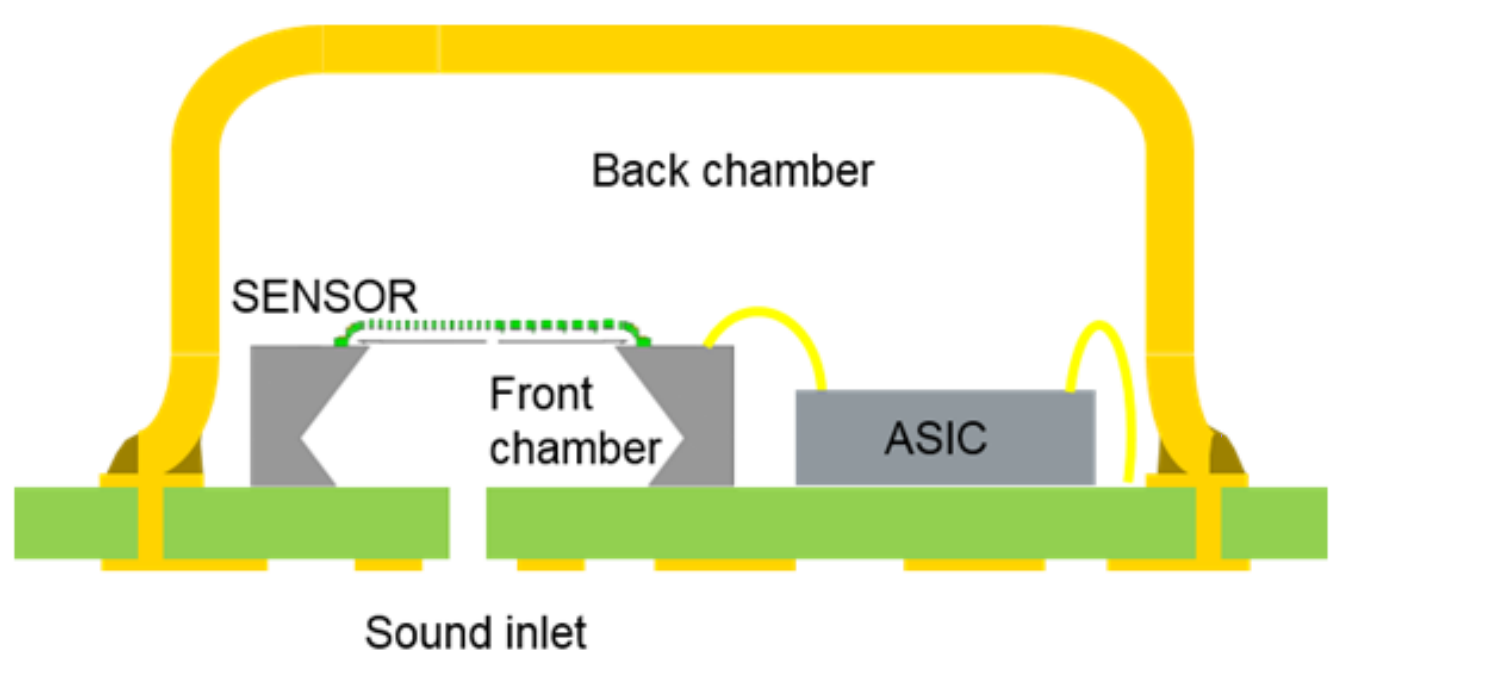
\includegraphics[width=0.5\textwidth]{thesistemplate/images/mems_schematic.png}
    \caption{MEMS Microphone schematic diagram with integrated ASIC \cite{mems_tutor}.}
    \label{fig:mems_schematic}
  \end{center}
\end{figure}



\subsubsection{I\textsuperscript{2}S communication interface}

The Inter-IC Sound (I\textsuperscript{2}S) bus protocol was developed by Philips in the late 1980s, as a constructive attempt for standardized communication of digital audio between electronic components. To minimize the number of pins required while keeping the protocol simple to decode, it uses a 3 lines serial bus: SD the Serial Data channel, WS or Word Select line, and SCK the Serial Clock line. In the data transmission, it is the master's task to generate the SCK and WS signals, in our case the STM32 microcontroller. The WS line indicates which channel (left or right) is being transmitted on the Data line, and it is changed one clock period before the MSB (Most Significant Bit).

The data provided by the I\textsuperscript{2}S slave microphone is 24-bit two's compliment MSB first, in Pulse Code Modulated (PCM) format. Since the sensor data precision is 18 bit only, the last 6 bits are always zeros and after the 24 bit sent the Data bus is changed to a high impedance(tri-state) state for the remaining part of the 32-bit data frame.

The selected sample rate is 16 kHz, similarly to most of the audio recordings used for training, even if higher sampling frequency options were supported, the additional higher resolution recordings have not been proven significantly beneficial during the testing, moreover it imposes considerable computational overhead.


\begin{figure}[h!]
  \begin{center}
    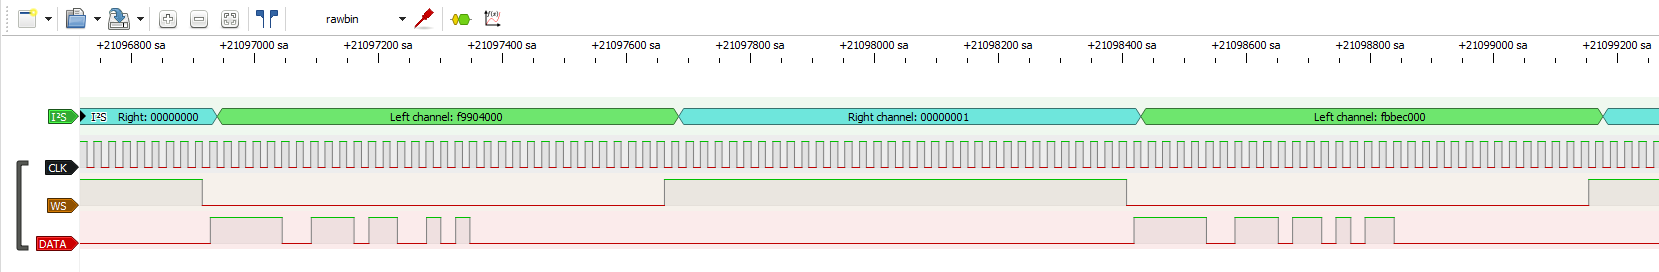
\includegraphics[width=1\textwidth]{thesistemplate/images/i2s_signal2.png}
    \caption{I\textsuperscript{2}S communication with Logic Analyzer and Protocol Decoder.}
    \label{fig:i2s_comm_prot_meas}
  \end{center}
\end{figure}

\begin{figure}[h!]
  \begin{center}
    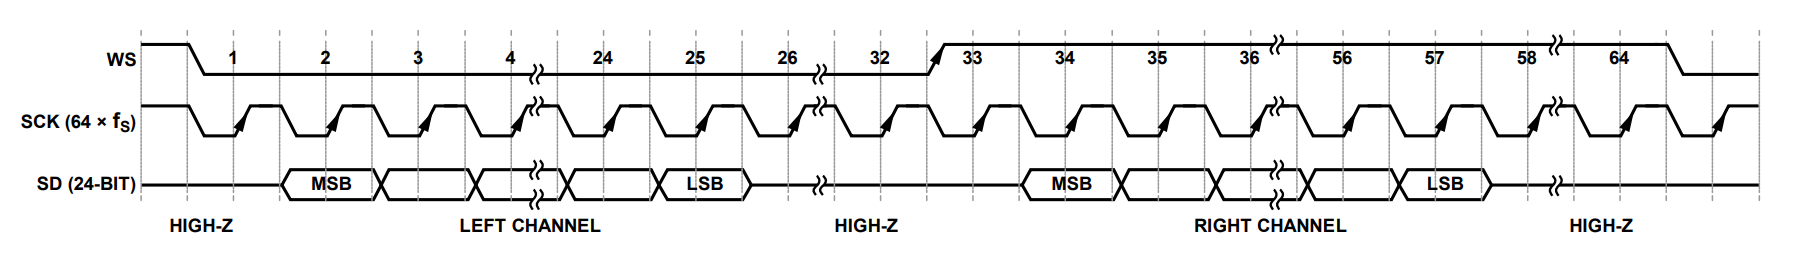
\includegraphics[width=1\textwidth]{thesistemplate/images/i2s_signal_datasheet.png}
    \caption{I\textsuperscript{2}S communication protocol example.}
    \label{fig:i2s_comm_prot}
  \end{center}
\end{figure}
% https://invensense.tdk.com/wp-content/uploads/2015/02/INMP441.pdf

% I2S specification, but we might need a better one for reference + the STM32 datasheet
% https://www.sparkfun.com/datasheets/BreakoutBoards/I2SBUS.pdf
% https://www.st.com/resource/en/reference_manual/dm00096844-stm32f401xbc-and-stm32f401xde-advanced-armbased-32bit-mcus-stmicroelectronics.pdf



\subsubsection{Audio DC component blocking filter}
\label{subsub:dc_blocking}

As elaborated in the datasheet of the chosen microphone MEMS microphone devices have a typical DC offset about 5 \% of the full range. Fortunately, the offset remains constant in the time frame of examination, therefore it is relatively easy to remove it without much distortion in the signal.

In the digital signal processing domain, various solutions exist for mitigating this problem. Keep tracking of a moving average and subtracting it from the audio stream is a straightforward approach and most resembles the process needed in the bias removal step of the data analysis. Based on research literature, it is a common practice to utilize a differentiator-integrator module to eliminate the DC component of a signal.

Exploiting the DSP capabilities of the STM microcontroller there is a simple and efficient way to implement a high-pass filter using the CMSIS DSP library. The task is to define the IIR filter parameters which fulfill the requirements. Second-order biquad filters are can be configured to execute the filtering in real-time on the audio stream. An example visualization of such filter is reported at \autoref{fig:biquad}.

In the discrete complex frequency domain, a DC blocking filter transfer function can be constructed with one pole and one zero and defined as:

\begin{equation}
   H(z) = \frac{Y(z)}{X(z)} = \frac{1-z^{-1}}{1-pz^{-1}} ,
\end{equation}

where the coefficient $p$ determines the cut off frequency and the system responsiveness. After cross multiplication, we get:

\begin{equation}
    Y(z)(1-pz^{-1}) = X(z)(1-z^{-1})  
\end{equation}


After removing the parentheses we can transform the equation to the discrete-time domain using common Z-transform pairs:

\begin{equation}
    y[n] - p\, y[n-1] = x[n] - x[n-1]
\end{equation}


\begin{equation}
    y[n]  = x[n] - x[n-1] + p\, y[n-1]
\end{equation}

Which now can be easily realized with a Single Biquad filter (IIR) efficiently, provided by the MCU hardware. The output of the filter in the discrete-time domain is given by the following equation:

\begin{equation}
y[n] = b_0 \, x[n] + b_1\,  x[n-1] + b_2\,  x[n-2] + a_1\,  y[n-1] + a_2\,  y[n-2]
\end{equation}

\begin{figure}[h!]
  \begin{center}
    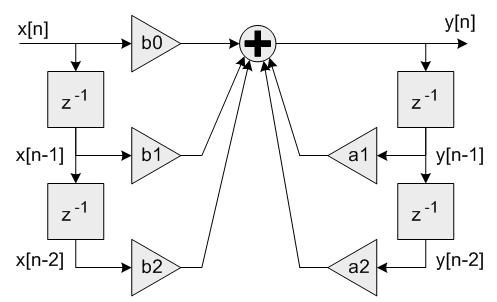
\includegraphics[width=0.5\textwidth]{thesistemplate/images/Biquad.png}
    \caption{Single Biquad filter provided by the CMSIS library.}
    \label{fig:biquad}
  \end{center}
\end{figure}

And finally from the last two equations the parameters can be inferred:


\begin{equation}
\label{eq:a_zero}
\begin{aligned}
a_1=p, b_0 = 1 \\
 a_2=0, b_1 = -1\\
b_2 = 0
\end{aligned}
\end{equation}

Recommendation for $p$ is provided by the microphone manufacturer for fixed and floating-point implementations \cite{knowles_dc_filter}. 

\begin{equation*}
    p = 1-2^{-12} \approx 0.99975586
\end{equation*}

% \begin{itemize}
%     \item TODO: Plot filter Bode diagram
% \end{itemize}

The effect of the filter on a short audio signal sample is demonstrated at \autoref{fig:dc_blocking_test}. Note that the simulation is plotted after the startup transition interval, in steady-state. No other additional filtering were added to the microphone signal. The DC-filtered signal will provide the basis for further signal processing steps related to feature extraction in frequency domain.

\begin{figure}[h!]
  \begin{center}
    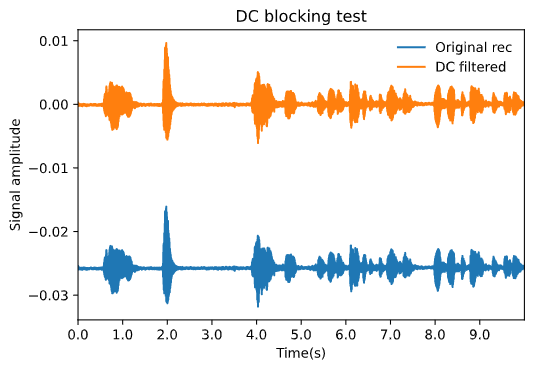
\includegraphics[width=0.7\textwidth]{thesistemplate/fig/dc_blocking.png}
    \caption{Testing the DC blocking filter functionality.}
    \label{fig:dc_blocking_test}
  \end{center}
\end{figure}



\subsubsection{PIR sensor}

The selection of a highly reliable and cost-effective motion sensor is also a key to the success of the project. After careful consideration of market alternatives, we have settled with the product portfolio provided by Panasonic. Their offering covers a wide variety of devices for different environments and signal output options. To simplify the development and match our design needs we have selected a digital PIR sensor (Panasonic EKMC167111) with a typical installation height of 3m with a relatively wide field of view (110$^{\circ}$) and 32 detection zones. The motion detection sensor will provide a logical high voltage level on the OUT pin in every situation when more than 4 $^{\circ}$C temperature difference is detected in two of the detection areas.

\begin{table}[h!]
\centering
\begin{tabular}{|l|l|}
\hline
\textbf{Parameter}                  & \textbf{Panasonic PIR EKMC}\\ \hline
Detection distance                  & up to 5 m                \\ \hline
Typical ceiling installation height & 3 m                      \\ \hline
Field of view                       & 110$^{\circ}$ $\times$ 110$^{\circ}$ \\ \hline
Detection zones                     & 32                       \\ \hline
Output type                         & Digital                  \\ \hline
Standby current consumption         & 170 \textmu A                 \\ \hline
\end{tabular}
\caption{Panasonic Digital PIR sensor specification summary \cite{papir_dsheet}.}
\end{table}

A cutaway diagram of a sample motion detector manufactured by Panasonic is shown at \autoref{fig:papir}. Unlike other companies on the market, their solutions include a tiny ASIC (Application Specific Integrated Circuit) inside the sensor case too, all integrated into a TO-5 sized metal can. The metal cover isolates the highly sensitive electronic components from electromagnetic fields caused by wireless devices, effectively preventing false alarms caused by interference. In the digital PIR sensors the ASIC performs differential signal amplification with an Operational amplifier coming from the analog Pyroelectric elements and implements a simple thresholding operation with a Comparator circuit. The output is a simple logical high or low voltage level based on the Comparator output. The spatial position and the number of detection zones are carefully controlled by the custom-designed Fresnel lens array on top of the sensing elements.

\begin{figure}[h!]
  \begin{center}
    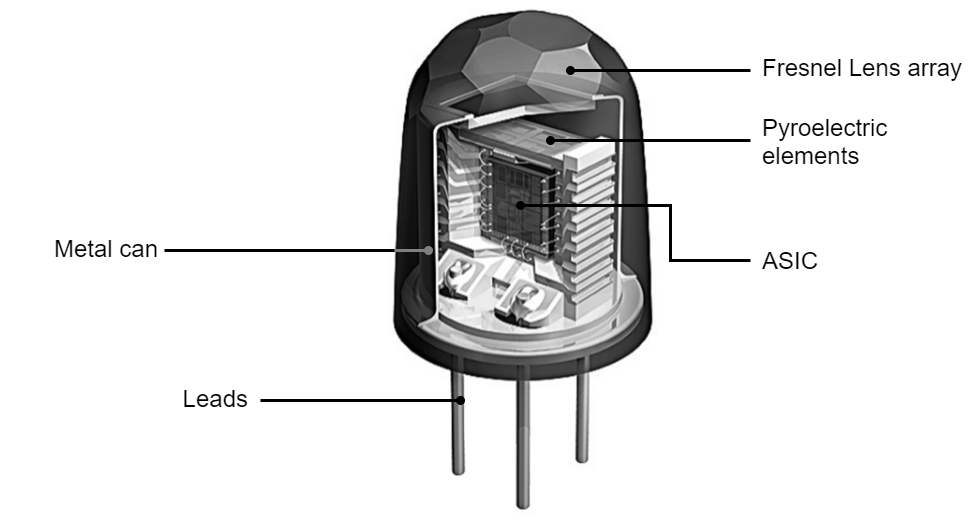
\includegraphics[width=0.9\textwidth]{thesistemplate/images/pir_cutaway.png}
    \caption{Panasonic PIR sensor cutaway diagram, adapted from the sensor datasheet \cite{papir_dsheet}.}
    \label{fig:papir}
  \end{center}
\end{figure}

% software
\section{Embedded Machine Learning model conversion and performance tests}

After when we found a feasible model structure that can also fulfill the requirements of the embedded platform we can convert the trained model to the MCU and run the inference to get real-time predictions. Dropout is removed during conversion by the STM32 provided X-Cube-AI tool, while conv and pool layers are fused by the tool for runtime-optimization reasons.


The handpicked best models from the previous chapter are tested by the following four performance measures:
\begin{itemize}
    \item[$-$] RAM memory requirements
    \item[$-$] Flash memory requirements
    \item[$-$] Execution time for inference
    \item[$-$] Complexity, MACC 
\end{itemize}

The performance tests serve also as a benchmark for the selected microcontroller platform to distinguish whether the available memory and computational power are sufficient to run a selected model inference in real-time. Additional resources need to be allocated to the audio feature extraction and other peripherals.

\subsection{RAM}

RAM is used only to store the intermediate (temporary) results during inference. The amount of space required for the application is excluded from the measurements. The same reserved memory block is used across different layers, reducing the size need. The RAM memory usage by layer can be examined for a selected network upon request.

\begin{figure}[h!]
  \begin{center}
    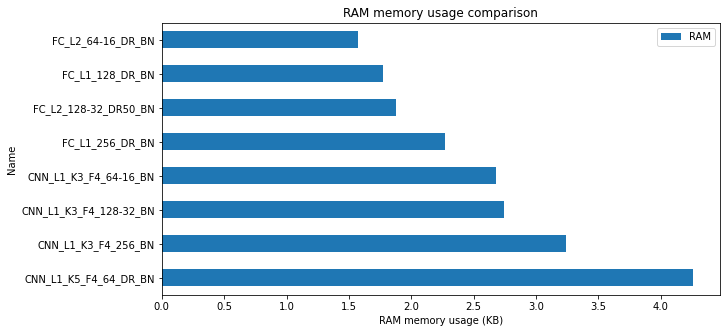
\includegraphics[width=1\textwidth]{thesistemplate/fig/ram_comp_emb.png}
    \caption{RAM memory requirements of the machine learning models tested.}
    \label{fig:ram_comp_emb}
  \end{center}
\end{figure}

Regarding the MCU limitations from the available 96 KB of RAM memory, even the largest one is just about 4.2 KB, consuming less than 5\% of the total memory space present.

\subsection{Flash}

The flash or ROM memory is used to store the weights and biases of the model. Additional space for the application was not included in the measurements. The model parameters and the compiled application code are written next to each other in the Flash memory space, but the reported values only representing the machine learning model memory needs.


\begin{figure}[h!]
  \begin{center}
    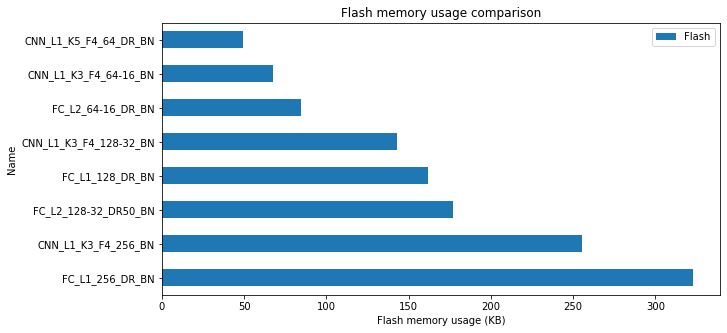
\includegraphics[width=1\textwidth]{thesistemplate/fig/flash_comp_emb.png}
    \caption{Flash memory requirements of the tested machine learning models tested.}
    \label{fig:flash_comp_emb}
  \end{center}
\end{figure}

Considering the total available flash space, 512 KB, larger models restrict the application by a large amount. The two largest models require 50\% and 65\% respectively, which might be a limiting factor for more complex problems.

\subsection{Inference time}

Inference time is measured as the total amount of time needed to propagate the input through the neural network and produce one output sequence.

\begin{figure}[h!]
  \begin{center}
    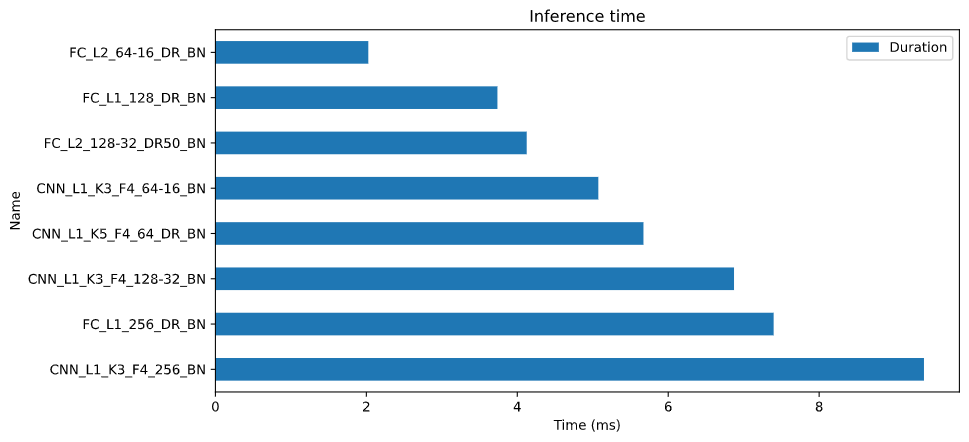
\includegraphics[width=1\textwidth]{thesistemplate/fig/inference_time.png}
    \caption{Inference time comparison for the machine learning models tested.}
    \label{fig:inference_time_comp_emb}
  \end{center}
\end{figure}

Examining the results depicted in \autoref{fig:inference_time_comp_emb} and running the microcontroller at 84 MHz, at its maximal speed, the inference process took less than 9 ms even in the most demanding scenario. As we will see in the following sections, this satisfies the real-time requirements for all of the selected models, since in the worst case one new column for the input needs to be computed in every 32 ms and about every 500 ms a new image will be constructed for inference.

\subsection{Complexity}

Complexity indicates the computational complexity of one inference process. It is common in embedded applications to approximate the complexity by the amount of Multiply And Accumulate (MACC) operations. The tests include an approximation of the activation functions and other general layers (Pooling, Batch Normalization) for the final estimations. 

On the selected M4 ARM chip each MACC operation takes is approximately 8 CPU cycles for FCN networks, while this value is slightly higher for CNN networks, around 12 in our test application. As it is visible on the results reported in \autoref{fig:complexity_comp_emb}, larger networks with more parameters generally require significantly more MACC operations, and the width of the fully connected layers are the most dominant influential factor.

\vspace{40px}

\begin{figure}[h!]
  \begin{center}
    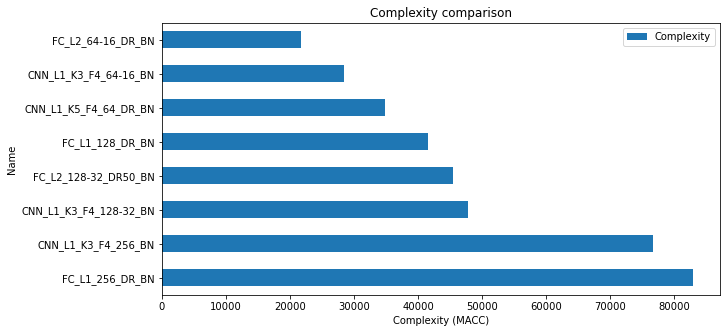
\includegraphics[width=1\textwidth]{thesistemplate/fig/complexity_comp_emb.png}
    \caption{Computational complexity comparison for the machine learning models tested.}
    \label{fig:complexity_comp_emb}
  \end{center}
\end{figure}


\section{Embedded AI process}

To benefit from the trained machine learning models on embedded we need to replicate the same data processing and feature extraction steps as in the PC version in python, but now in Embedded C, in a highly resource-constrained environment.

The data collection and preprocessing steps until the two-dimensional MFCC image construction are summarized in \autoref{fig:embedded_ai_proc}. To provide an instantaneous response to the final user the audio flow and the feature computation are continuous yielding one new occupancy prediction in each 500 ms.

The process starts with data fetching from the microphone. The audio sampling rate was kept at 16 kHz and 18-bit PCM samples were transferred through one of the I2S buses of the microcontroller in 32-bit frames. On the whole, the audio stream from one mic produces 62.5 KB/s of constant data flow, which if handled by the CPU, would have consumed most of its resources only just to move the data from peripheral to memory. Fortunately, the task can be outsourced to one of the two Direct Memory Access (DMA) controllers of the MCU, alleviating the need for CPU-based data movement. The DMA gets assigned to a fixed size of memory at the initialization step and during runtime, it keeps copying new samples to a circular buffer. The CPU will get notified through an interrupt request when the buffer is at half-full and full state, signaling the moment for the start of the signal processing tasks. By design, the size of the DMA input buffer is matching the number of samples needed to calculate one set of MFCC features, which is 512 samples, representing 32 ms of audio.

After when we have one set of 18 bit PCM coded audio first we convert it to 32-bit floating-point numbers, then we apply the IIR filter designed in section \ref{subsub:dc_blocking} for the DC offset removal. Now, the signal is ready for MFCC feature extraction. Following the pattern with the python-based solution, 21 MFCC features are extracted with the same additional parameters for Fourier-transformation, with the zeroth coefficient discarded. The MFCC features are computed with the help of the Audio Preprocessing library provided by STM32.

The 20 MFCC features give one column of the input image for the machine learning model, so the process described above must be repeated a total of 16 times to construct a final 20$\times$16 shaped array to match the input specification. After propagating the full array through the neural network we will get one prediction for audio-based presence.



\begin{figure}[h!]
  \begin{center}
    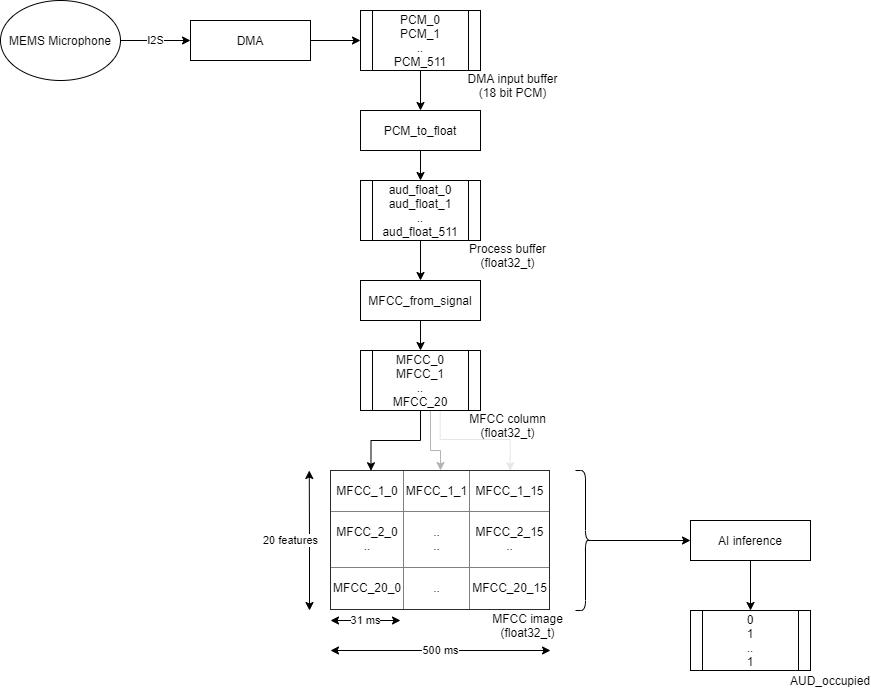
\includegraphics[width=0.9\textwidth]{thesistemplate/fig/embedded_aud_proces.png}
    \caption{Embedded AI preprocessing and inference flowchart, once only one column of the MFCC image is computed. For one AI inference step 16 consecutive columns need to be stored, this indicated with different shades of gray arrows above the MFCC image.}
    \label{fig:embedded_ai_proc}
  \end{center}
\end{figure}


\section{Sensor output fusion with State Machine}

The last step to form a multisensory room occupancy device prototype is to merge the audio-based predictions from the machine learning model and the signals from the PIR motion detection sensor. Since the PIR sensor already provides a digital output when movement is detected, no additional signal processing was applied to the sensor output. After the corresponding pin is configured as digital input on the MCU, each time a rising edge occurs (change in value from 0 to 1), it will trigger a dedicated GPIO interrupt request (EXTI\_IRQ) which is then handled by software callbacks.

An essential question in the design of the fusion algorithm is, whether what is the relative importance of each sensor prediction in various situations and how to form a framework that can incorporate these subtle differences. On an empirical basis, PIR sensors can reliably detect when someone entered the room (high True Positive rate) and have few or no false triggers when the room is empty (high True Negative rate). From a user experience point of view, False-negative predictions are the most visible, unpleasant misbehavior, which needs additional correction. Namely, the situations after one goes into a room, get recognized by the PIR first, but if she stays there seated, the sensor could miss the small movements and falsely predicting an empty room. The introduction of another information source in these states can improve the overall experience by a large amount.
Moreover, preliminary tests with the sound-based classification suggest that microphone or unexpected noises can trigger the model in some situations generating random false positive samples.

Considering the sensor differences a weighted sum of the outputs was constructed, referred to as confidence from now on. The confidence is a value from 0 to 100\%, indicating the confidence in the prediction that one or multiple persons are using the room. If no reinforcement comes from the sensors the value is decreasing linearly. The rate is configurable to imitate more or less aggressive light switching behavior. The default value for the demo is a 5\% decrease every second. The PIR sensor trigger immediately boosts the confidence up to 100\% and one sound-based prediction adds 10\% to the total confidence value.

The designed State machine transition diagram is shown at \autoref{fig:state_mach}. The two states are the Occupied and the Unoccupied room states and the transition between them is based on the current confidence value. As it is visible on the image the two state transition values are 60\% and 40\%, which creates a hysteresis effect, making the transition more reliable from an outside perspective.



\begin{figure}[ht!]
  \begin{center}
    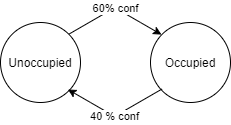
\includegraphics[width=0.4\textwidth]{thesistemplate/images/state_mach.png}
    \caption{State machine transition diagram based on confidence values.}
    \label{fig:state_mach}
  \end{center}
\end{figure}


\begin{figure}[h!]
  \begin{center}
    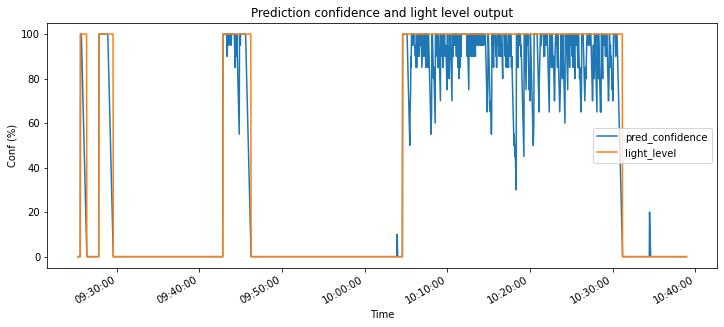
\includegraphics[width=1\textwidth]{thesistemplate/fig/conf_with_lights2.png}
    \caption{Room occupancy confidence with controlled light level values.}
    \label{fig:conf_with_lights}
  \end{center}
\end{figure}